\chapter{Visão geral da arquitetura}

\begin{chapquote}{Autor desconhecido}
``Aviso, teclado não encontrado. Pressione Enter para continuar.''
\end{chapquote}

Este capítulo apresenta uma visão geral básica da arquitetura \textbf{x86-64}. Para uma explicação mais detalhada, consulte as referências adicionais observadas no Capítulo \ref{cap1}, Introdução.

\section{Visão geral da arquitetura}
Os componentes básicos de um computador incluem uma unidade de processamento central (CPU), armazenamento primário ou memória de acesso aleatório (RAM), armazenamento secundário, dispositivos de entrada/saída (por exemplo, tela, teclado, mouse) e uma interconexão conhecida como barramento.

Um diagrama básico da arquitetura do computador é a da Figura \ref{arquiteturacomputador}:
\begin{figure}[ht]
	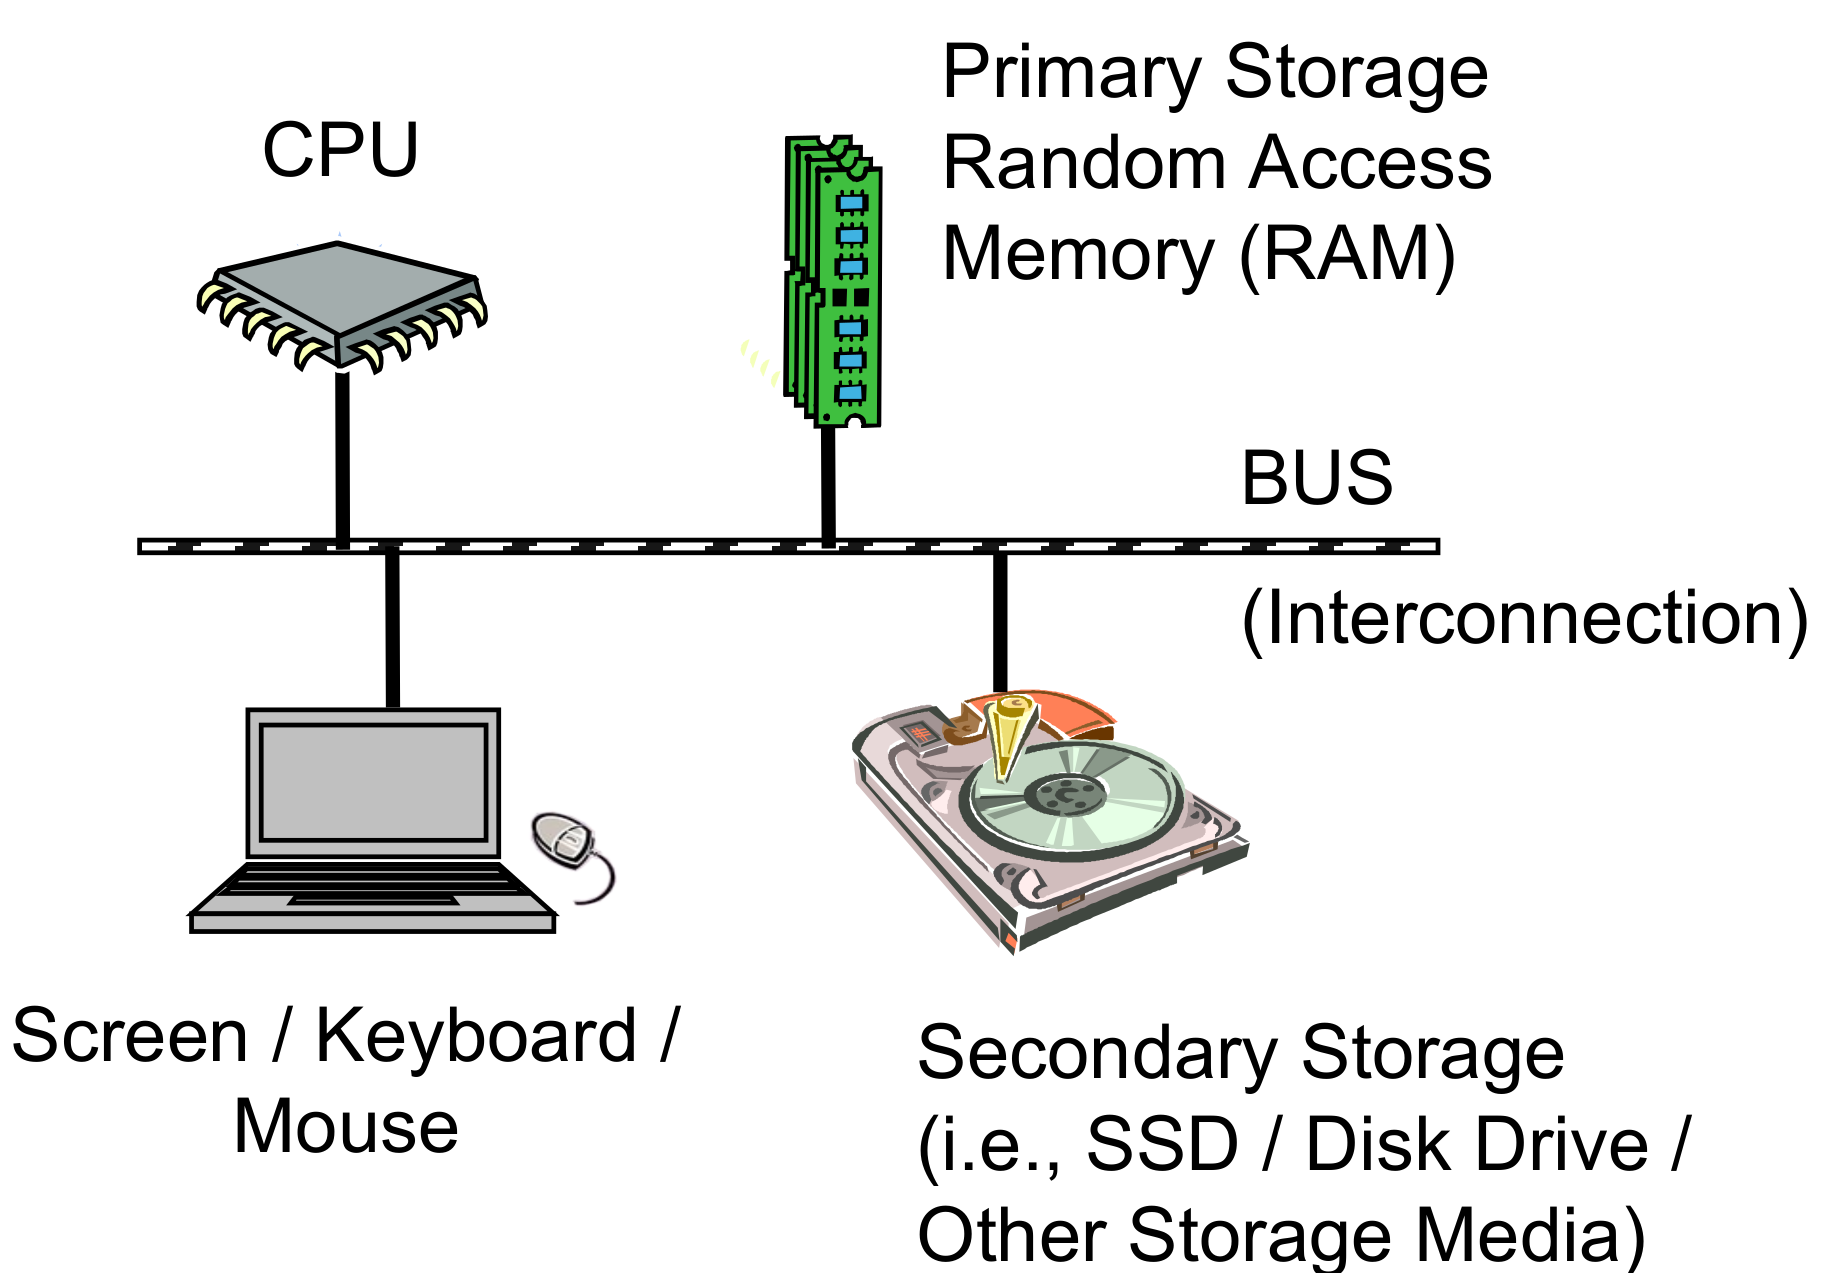
\includegraphics[width=\linewidth]{imagens/arquitetura}
	\caption{Arquitetura de um computador}
	\label{arquiteturacomputador}
\end{figure}

A arquitetura é normalmente conhecida como Arquitetura Von Neumann\footnote{Para obter mais informações, consulte: https://pt.wikipedia.org/wiki/Arquitetura\_de\_von\_Neumann}, ou arquitetura Princeton, e foi descrita em 1945 pelo matemático e físico John von Neumann.

Programas e dados são normalmente armazenados em armazenamento secundário (por exemplo, unidade de disco ou unidade de estado sólido). Quando um programa é executado, ele deve ser copiado do armazenamento secundário para o armazenamento primário ou memória principal (RAM). A CPU executa o programa a partir do armazenamento primário ou RAM.

O armazenamento primário ou memória principal também é conhecido como \textit{memória volátil}, pois quando a energia é removida, a informação não é retida e, portanto, perdida. O armazenamento secundário é conhecido como \textit{memória não volátil}, uma vez que as informações são retidas quando desligadas.

Por exemplo, considere armazenar um trabalho de conclusão de curso em armazenamento secundário (ou seja, disco). Quando o usuário começa a escrever ou editar o trabalho de conclusão de curso, ele é copiado do meio de armazenamento secundário para o armazenamento primário (isto é, RAM ou memória principal). Quando concluído, a versão atualizada normalmente é armazenada de volta no armazenamento secundário (ou seja, disco). Se você já perdeu energia durante a edição de um documento (presumindo que não há bateria ou fonte de alimentação ininterrupta), perder o trabalho não salvo certamente esclarecerá a diferença entre memória volátil e não volátil.

\section{Tamanhos de armazenamento de dados}
A arquitetura x86-64 oferece suporte a um conjunto específico de elementos de tamanho de armazenamento de dados, todos baseados em potências de dois. Os tamanhos de armazenamento suportados são os da Tabela \ref{tab:tamanhosdearmazenamento}:

\begin{table}[h]
	\centering
	\begin{tabular}{|l|c|c|}
		\hline
		\rowcolor[HTML]{C0C0C0} 
		{\color[HTML]{000000} } Armazenamento & {\color[HTML]{000000} Tamanho (bits)} & {\color[HTML]{000000} Tamanho (bytes)} \\ \hline
		Byte& 8 bits & 1 byte\\ \hline
		Word & 16 bits & 2 bytes\\ \hline
		Double-word & 32 bits & 4 bytes\\ \hline
		Quadword & 64 bits & 8 bytes\\ \hline
		Double quadword & 128 bits & 16 bytes  \\ \hline
	\end{tabular}
	\caption{Tamanhos de armazenamento.}
	\label{tab:tamanhosdearmazenamento}
\end{table}

Listas ou arrays (conjuntos de memória) podem ser reservados em qualquer um desses tipos.

Esses tamanhos de armazenamento têm uma correlação direta com as declarações de variáveis em linguagens de alto nível (por exemplo, C, C ++, Java, etc.).

Por exemplo, as declarações C/C ++ são mapeadas da seguinte maneira:
\begin{table}[h]
	\centering
	\begin{tabular}{|l|l|c|c|}
		\hline
		\rowcolor[HTML]{C0C0C0} 
		{\color[HTML]{000000} } Declaração em C/C++ & {\color[HTML]{000000} Armazenamento} & {\color[HTML]{000000} Tamanho (bits)} & {\color[HTML]{000000} Tamanho (bytes)} \\ \hline
		char & Byte& 8 bits & 1 byte\\ \hline
		short & Word & 16 bits & 2 bytes\\ \hline
		int & Double-word & 32 bits & 4 bytes\\ \hline
		unsigned int & Double-word & 32 bits & 4 bytes\\ \hline
		long\footnotemark & Quadword & 64 bits & 8 bytes\\ \hline
		long long  & Quadword & 64 bits & 8 bytes\\ \hline
		char *  & Quadword & 64 bits & 8 bytes\\ \hline
		int * & Quadword & 64 bits & 8 bytes\\ \hline
		float & Double quadword & 128 bits & 16 bytes  \\ \hline
		double & Double quadword & 128 bits & 16 bytes  \\ \hline
	\end{tabular}

	\caption{Declarações em C/C++.}
	\label{tab:declaracoesemC}
\end{table}
\footnotetext[2]{Observe que a declaração do tipo 'long' depende do compilador. O tipo mostrado é para compiladores gcc e g ++.}

O asterisco indica uma variável de endereço. Por exemplo, \textbf{int *} significa o endereço de um inteiro. Outras linguagens de alto nível geralmente têm mapeamentos semelhantes.

\section{Unidade central de processamento}
A \textbf{Unidade de Processamento Central}\footnote{Para obter mais informações, consulte: https://pt.wikipedia.org/wiki/Unidade\_central\_de\_processamento} (CPU) é normalmente referida como o ``cérebro'' do computador, uma vez que é onde os cálculos reais são realizados. A CPU está alojada em um único chip, às vezes chamado de processador, chip ou \textit{die}\footnote{Para obter mais informações, consulte: https://pt.wikipedia.org/wiki/Die\_(circuito\_integrado)}. A imagem da capa mostra tal CPU.

O chip da CPU inclui várias unidades funcionais, incluindo a Unidade Lógica e Aritmética\footnote{Para obter mais informações, consulte: https://pt.wikipedia.org/wiki/Unidade\_lógica\_e\_aritmética} (ULA), que é a parte do chip que realmente executa os cálculos aritméticos e lógicos. Para dar suporte à ULA, os registros do processador\footnote{Para obter mais informações, consulte: https://pt.wikipedia.org/wiki/Registrador\_(informática)} e a memória cache\footnote{Para obter mais informações, consulte: https://pt.wikipedia.org/wiki/Cache} também estão incluídos `no dado''` (termo para dentro do chip). Os registros da CPU e a memória cache são descritos nas seções subsequentes.

\subsection{Registradores da CPU}
Um registrador da CPU, ou apenas registrador, é um armazenamento temporário ou local de trabalho embutido na própria CPU (separado da memória). Os cálculos são normalmente executados pela CPU usando registradores.

\subsubsection{Registradores de uso geral (GPRs)}
Existem dezesseis registradores de uso geral (General Purpose Registers - GPRs) de 64 bits. Os GPRs são descritos na tabela a seguir. Um registro GPR pode ser acessado com todos os 64 bits ou alguma parte ou subconjunto acessado (vide Tabela \ref{tab:registradores}).

\begin{table}[h]
	\centering
	\begin{tabular}{|c|c|c|c|}
		\hline
		\rowcolor[HTML]{C0C0C0} 
		Registrador & 32 bits & 16 bits & 8 bits \\ 
		\rowcolor[HTML]{C0C0C0} 
		de 64 bits & mais baixos & mais baixos & mais baixos \\ \hline
		rax & eax& ax & al\\ \hline
		rbx & ebx& bx & bl\\ \hline
		rcx & ecx& cx & cl\\ \hline
		rdx & edx& dx & dl\\ \hline
		rsi & esi& si & sil\\ \hline
		rdi & edi& di & dil\\ \hline
		rbp & ebp& bp & bpl\\ \hline
		rsp & esp& sp & spl\\ \hline
		r8 & r8d& r8w & r8b\\ \hline
		r9 & r9d& r9w & r9b\\ \hline
		r10 & r10d& r10w & r10b\\ \hline
		r11 & r11d& r11w & r11b\\ \hline
		r12 & r12d& r12w & r12b\\ \hline
		r13 & r13d& r13w & r13b\\ \hline
		r14 & r14d& r14w & r14b\\ \hline
		r15 & r15d& r15w & r15b\\ \hline
	\end{tabular}
	
	\caption{Registradores da CPU.}
	\label{tab:registradores}
\end{table}

Além disso, alguns dos registradores GPR são usados para fins específicos, conforme descrito nas seções posteriores.

Ao usar tamanhos de elementos de dados menores que 64 bits (ou seja, 32 bits, 16 bits ou 8 bits), a parte inferior do registro pode ser acessada usando um nome de registro diferente, conforme mostrado na tabela.

Por exemplo, ao acessar as partes inferiores do registrador \textbf{rax} de 64 bits, o layout é o seguinte:

\begin{figure}[ht]
	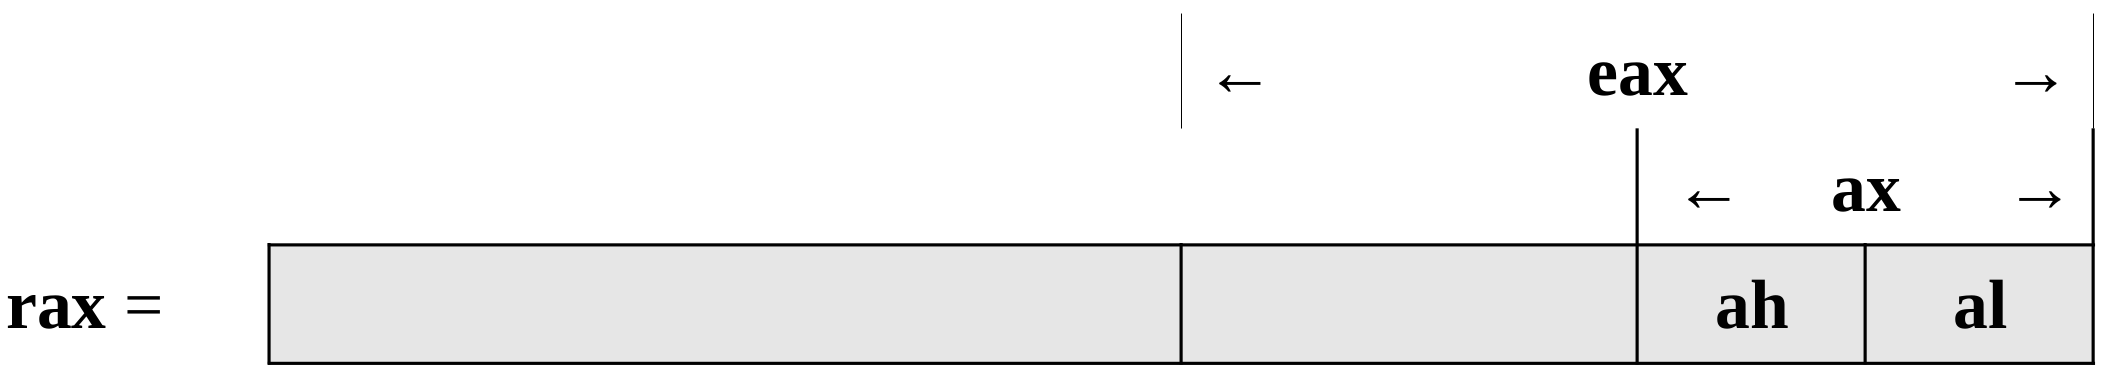
\includegraphics[width=0.8\linewidth]{imagens/layoutrax}
	\caption{Layout do registrador rax.}
	\label{layoutrax}
\end{figure}

Conforme mostrado no diagrama, os primeiros quatro registros, \textbf{rax}, \textbf{rbx}, \textbf{rcx} e \textbf{rdx} também permitem que os bits 8-15 sejam acessados com os nomes de registro \textbf{ah}, \textbf{bh}, \textbf{ch} e \textbf{dh}. Com exceção de \textbf{ah}, eles são fornecidos para suporte de legado e não serão usados neste texto.

A capacidade de acessar partes do registro significa que, se o registro quadword \textbf{rax}  for definido como $ 50.000.000.000_{10} $ (cinquenta bilhões), o registro \textbf{rax} conterá o seguinte valor em \textit{hex}.

\begin{center}
	\textbf{rax = 0000 000B A43B 7400}
\end{center}

Se uma operação subsequente definir o registro da palavra \textbf{ax} para $ 50.000_{10} $ (cinquenta mil, que é $ C350_{16} $), o registro \textbf{rax} conterá o seguinte valor em \textit{hex}.

\begin{center}
	\textbf{rax = 0000 000B A43B C350}
\end{center}

Nesse caso, quando a parte inferior \textbf{ax} de 16 bits do registrador \textbf{rax} de 64 bits é definida, os 48 bits superiores não são afetados. Observe a mudança no \textbf{AX} (de $ 7400_{16} $ para $ C350_{16} $).

Se uma operação subsequente definir o registro \textbf{al} de tamanho de byte para $ 50_{10} $ (cinquenta, que é $ 32_{16} $), o registro \textbf{rax} conterá o seguinte valor em hexadecimal.

\begin{center}
	\textbf{rax = 0000 000B A43B C332}
\end{center}

Quando a parte inferior \textbf{al} de 8 bits do registro \textbf{rax} de 64 bits é definida, os 56 bits superiores não são afetados. Observe a mudança em \textbf{AL} (de $ 50_{16} $ para $ 32_{16}$).

Para operações de registrador de 32 bits, os 32 bits superiores são apagados (definidos para zero). Geralmente, isso não é um problema, pois as operações em registradores de 32 bits não usam os 32 bits superiores do registrador. Para valores não sinalizados, isso pode ser útil para converter de 32 bits para 64 bits.
No entanto, isso não funcionará para conversões sinalizadas de valores de 32 bits para 64 bits.
Especificamente, ele fornecerá resultados potencialmente incorretos para valores negativos de números.
Consulte o Capítulo \ref{cap:representacaodedados}, \textit{Representação de dados}, para obter informações adicionais sobre a representação de valores com sinais.

\subsubsection{Stack Pointer Register (RSP)}
Um dos registradores da CPU, \textbf{rsp}, é usado para apontar para o topo atual da pilha. O registrador \textbf{rsp} não deve ser usado para dados ou outros usos. Informações adicionais sobre as operações de pilha e pilha são fornecidas no Capítulo \ref{cap:pilhadeprocessos}, Pilha de processos.

\subsubsection{Base Pointer Register (RBP)}
Um dos registradores da CPU, \textbf{rbp}, é usado como um ponteiro base durante as chamadas de função. O registro \textbf{rbp} não deve ser usado para dados ou outros usos. Informações adicionais sobre as funções e chamadas de função são fornecidas no Capítulo \ref{cap:Funções}, Funções.


\subsubsection{Instruction Pointer Register (RIP)}
Além dos GPRs, existe um registro especial, \textbf{rip}, que é usado pela CPU para apontar a próxima instrução a ser executada. Especificamente, uma vez que o \textbf{rip} aponta para a próxima instrução, isso significa que a instrução apontada por \textbf{rip} e mostrada no depurador ainda não foi executada. Esta é uma distinção importante que pode ser confusa ao revisar o código em um depurador.

\subsubsection{Flag Register (rFlags)}
O registrador de sinalização, \textbf{rFlags}, é usado para informações de status e controle da CPU. O registro \textbf{rFlag} é atualizado pela CPU após cada instrução e não pode ser acessado diretamente pelos programas. Este registro armazena informações de status sobre a instrução que acabou de ser executada. Dos 64 bits do registrador \textbf{rFlag}, muitos são reservados para uso futuro.

A Tabela \ref{tab:flags} mostra alguns dos bits de status no registrador de sinalizador.

\begin{table}[h]
	\centering
	\begin{tabular}{|c|c|c|l|}
		\hline
		\rowcolor[HTML]{C0C0C0} 
		\textbf{Nome} & \textbf{Símbolo} & \textbf{Bit} & \textbf{Uso} \\ 
		Carry & CF & 0  & Usado para indicar se a operação anterior\\
		& & & resultou em um transporte (vai um).\\ \hline
		Paridade & PF& 2 & Usado para indicar se o último byte tem\\
		& & &  um número par de 1 (ou seja, paridade par).\\ \hline
		Ajuste & AF& 4 & Usado para suportar operações decimais\\
		& & &  codificadas binárias.\\ \hline
		Zero & ZF& 6 & Usado para indicar se a operação anterior\\
		& & &  resultou em um resultado zero.\\ \hline
		Sinal & SF& 7 & Utilizado para indicar se o resultado\\
		& & &  da operação anterior resultou em 1 no bit\\
		& & &  mais significativo (indicando negativo no\\
		& & &  contexto de dados sinalizados).\\ \hline
		Direção & DF& 10 & Usado para especificar a direção (incremento\\
		& & &  ou decremento) para algumas operações de\\
		& & &  string.\\ \hline
		Overflow & OF& 11 & Usado para indicar se a operação anterior\\
		& & &  resultou em um estouro.\\ \hline
	\end{tabular}
	
	\caption{Flags.}
	\label{tab:flags}
\end{table}

Existem vários bits adicionais não especificados neste texto. Mais informações podem ser obtidas nas referências adicionais observadas no Capítulo \ref{cap1}, \textit{Introdução}.

\subsubsection{Registradores XMM}
Há um conjunto de registradores dedicados usados para oferecer suporte a operações de ponto flutuante de 64 e 32 bits e instruções de Single Instruction Multiple Data (SIMD). As instruções \textbf{SIMD} permitem que uma única instrução seja aplicada simultaneamente a vários itens de dados. Usado de forma eficaz, isso pode resultar em um aumento significativo de desempenho. As aplicações típicas incluem algum processamento gráfico e processamento de sinal digital.

Os registradores \textbf{XMM} são apresentados na Tabela \ref{tab:xmm}.


\begin{table}[h]
	\centering
	\begin{tabular}{|c|}
		\hline
		\rowcolor[HTML]{C0C0C0} 
		\textbf{Registradores de 128 bits} \\ \hline
		xmm0 \\ \hline
		xmm1 \\ \hline
		xmm2 \\ \hline
		xmm3 \\ \hline
		xmm4 \\ \hline
		xmm5 \\ \hline
		xmm6 \\ \hline
		xmm7 \\ \hline
		xmm8 \\ \hline
		xmm9 \\ \hline
		xmm10 \\ \hline
		xmm11 \\ \hline
		xmm12 \\ \hline
		xmm13 \\ \hline
		xmm14 \\ \hline
		xmm15 \\ \hline
	\end{tabular}
	
	\caption{Registradores xmm.}
	\label{tab:xmm}
\end{table}

Observe que alguns dos processadores X86-64 mais recentes suportam registros \textbf{XMM} de 256 bits. Isso não será uma questão para os programas neste texto.

Além disso, os registradores \textbf{XMM} são usados para oferecer suporte a \textit{Streaming SIMD Extensions} (SSE). As instruções \textbf{SSE} estão fora do escopo deste texto. Mais informações podem ser obtidas nas referências da Intel (conforme observado no Capítulo \ref{cap1}, \textit{Introdução}).

\subsection{Memória cache}
A memória cache é um pequeno subconjunto do armazenamento primário ou RAM localizado no chip da CPU. Se um local de memória for acessado, uma cópia do valor é colocada no cache. Os acessos subsequentes a esse local da memória que ocorrem em rápida sucessão são recuperados do local do cache (interno ao chip da CPU). Uma leitura de memória envolve o envio do endereço por meio do barramento para o controlador de memória, que obterá o valor no local de memória solicitado e o enviará de volta pelo barramento. Comparativamente, se um valor estiver no cache, será muito mais rápido acessar esse valor.

Um \textbf{acerto} de cache ocorre quando os dados solicitados podem ser encontrados em um cache, enquanto uma \textbf{falha} de cache ocorre quando não pode. As ocorrências de cache são atendidas pela leitura de dados do cache, o que é mais rápido do que ler da memória principal. Quanto mais solicitações podem ser atendidas do cache, mais rápido o sistema normalmente executará. Gerações sucessivas de chips de CPU aumentaram a memória cache e aprimoraram as estratégias de mapeamento de cache para melhorar o desempenho geral.

Um diagrama de blocos de uma configuração típica de chip de CPU é o dada na Figura \ref{fig:cache} :
\begin{figure}[ht]
\begin{center}
		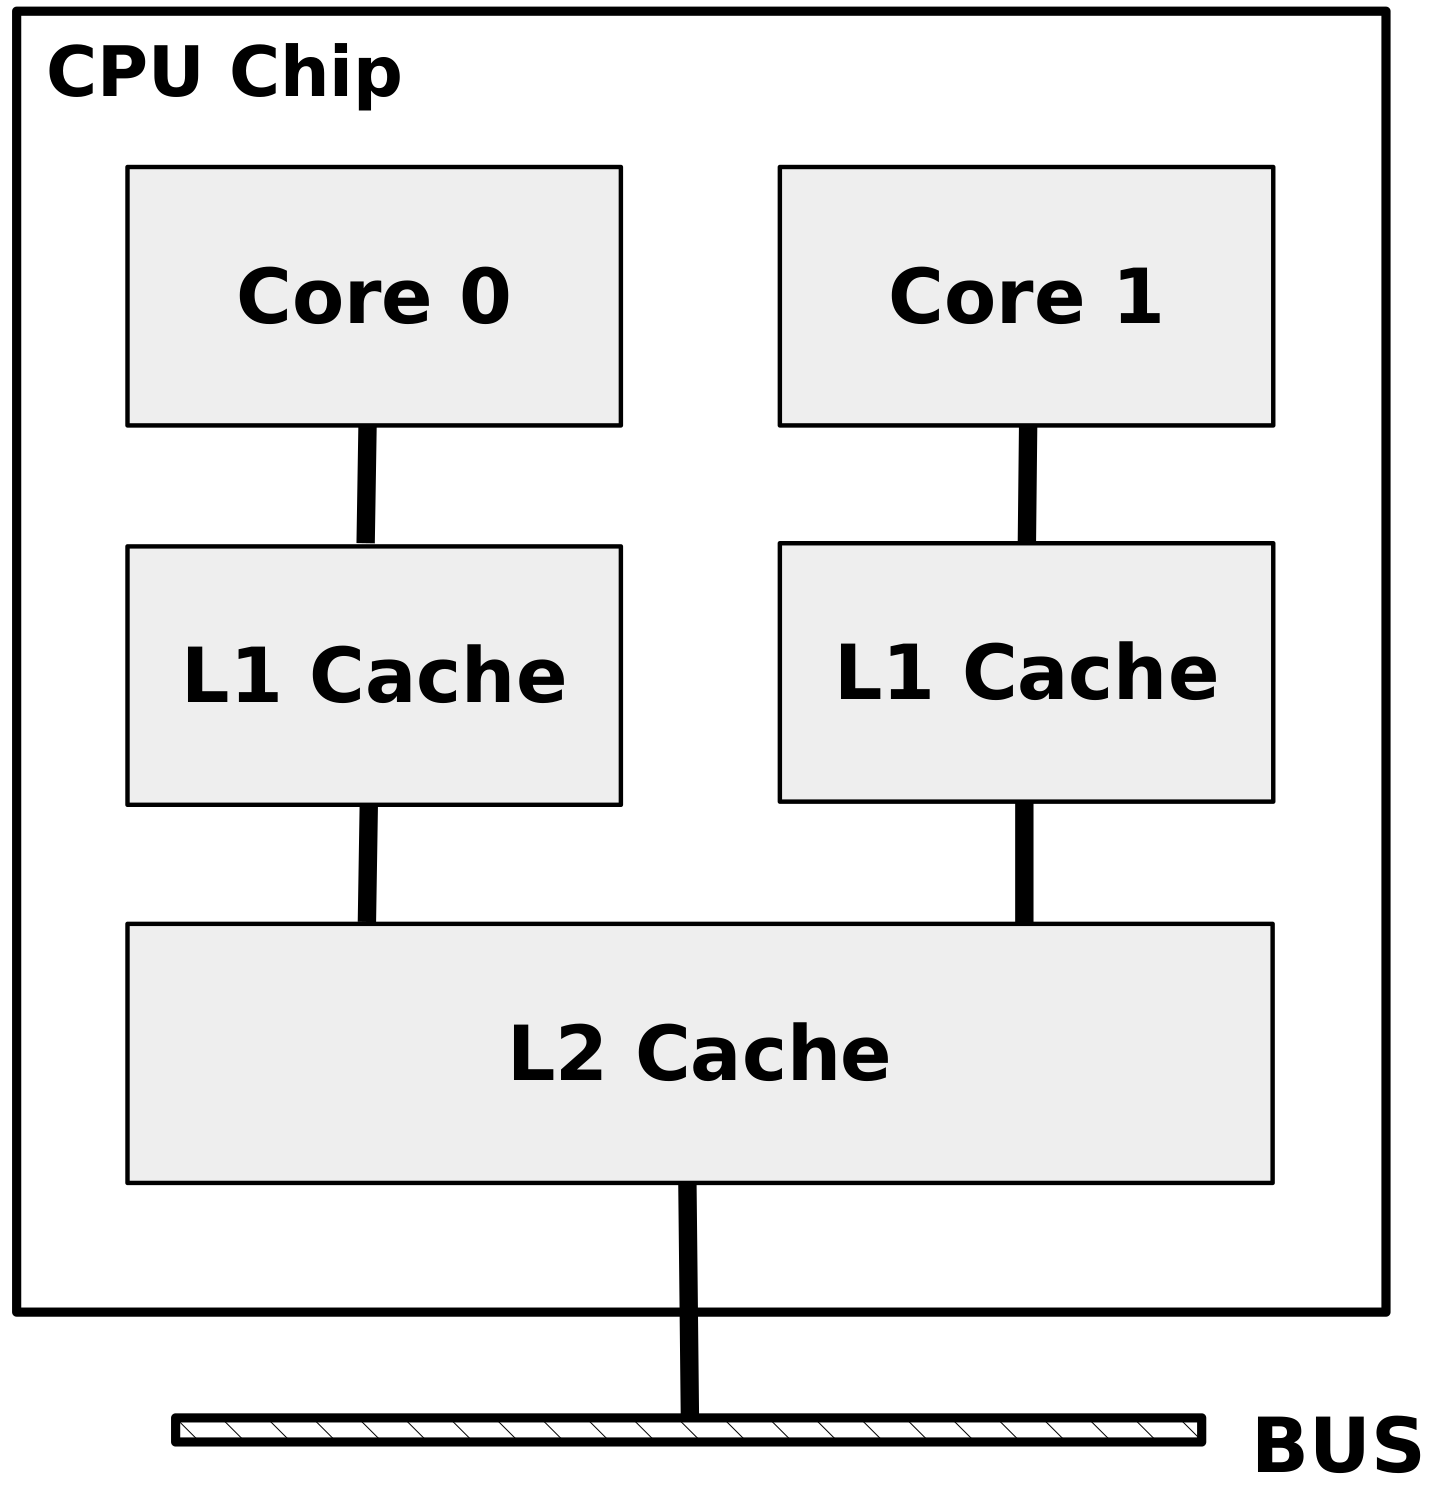
\includegraphics[width=0.8\linewidth]{imagens/cache}
\end{center}
	\caption{Diagrama em blocos de memória cache}
	\label{fig:cache}
\end{figure}

Os designs de chip atuais normalmente incluem um cache \textbf{L1} por núcleo e um cache \textbf{L2} compartilhado. Muitos dos chips de CPU mais recentes terão um cache \textbf{L3} adicional.

Como pode ser observado no diagrama, todos os acessos à memória passam por cada nível de cache. Como tal, há um potencial para cópias múltiplas e duplicadas do valor (registro de CPU, cache L1, cache L2 e memória principal). Essa complicação é gerenciada pela CPU e não é algo que o programador possa alterar. Compreender o cache e o ganho de desempenho associado é útil para entender como um computador funciona.

\section{Memória principal}
A memória pode ser vista como uma série de bytes, um após o outro. Ou seja, a memória é endereçável por byte. Isso significa que cada endereço de memória contém um byte de informação. Para armazenar uma palavra dupla, são necessários quatro bytes que usam quatro endereços de memória.

Além disso, a arquitetura é \textbf{little-endian}. Isso significa que o Byte menos significativo (\textit{Least Significant Byte}, LSB)) é armazenado no endereço de memória mais baixo. O Byte mais significativo (\textit{Most Significant Byte}, MSB) é armazenado no local de memória mais alto.

Para uma palavra dupla (32 bits), o MSB e o LSB são alocados conforme mostrado na Figura \ref{fig:msb}.
\begin{figure}[ht]
	\begin{center}
		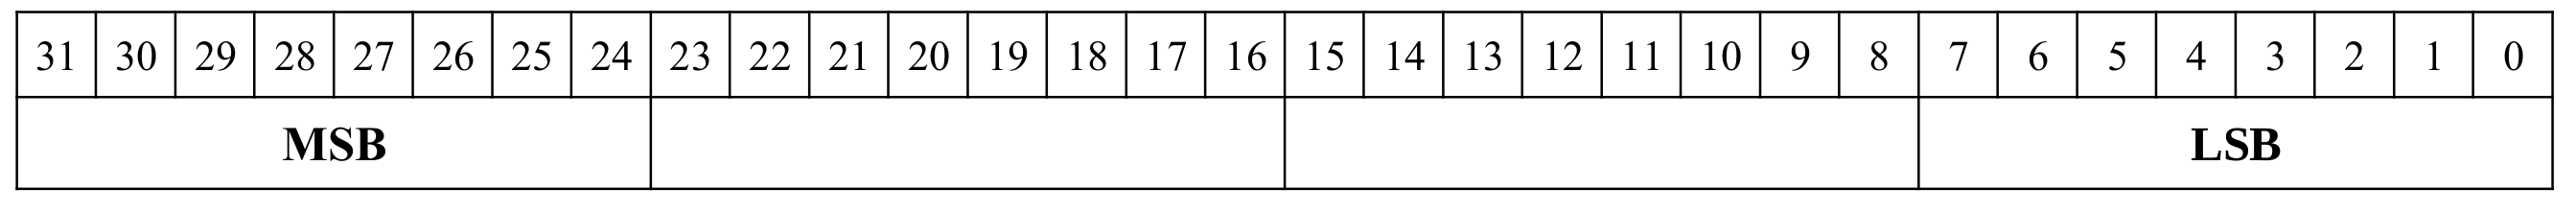
\includegraphics[width=\linewidth]{imagens/msb}
	\end{center}
	\caption{MSB e LSB}
	\label{fig:msb}
\end{figure}

Por exemplo, assumindo o valor de $ 5.000.000_{10} $ ($ 004C4B40_{16} $), deve ser colocado em uma variável de palavra dupla chamada \textbf{var1}.

Para uma arquitetura \textit{little-endian}, a imagem da memória seria a da Figura \ref{fig:littleendien}:
\begin{figure}[ht]
	\begin{center}
		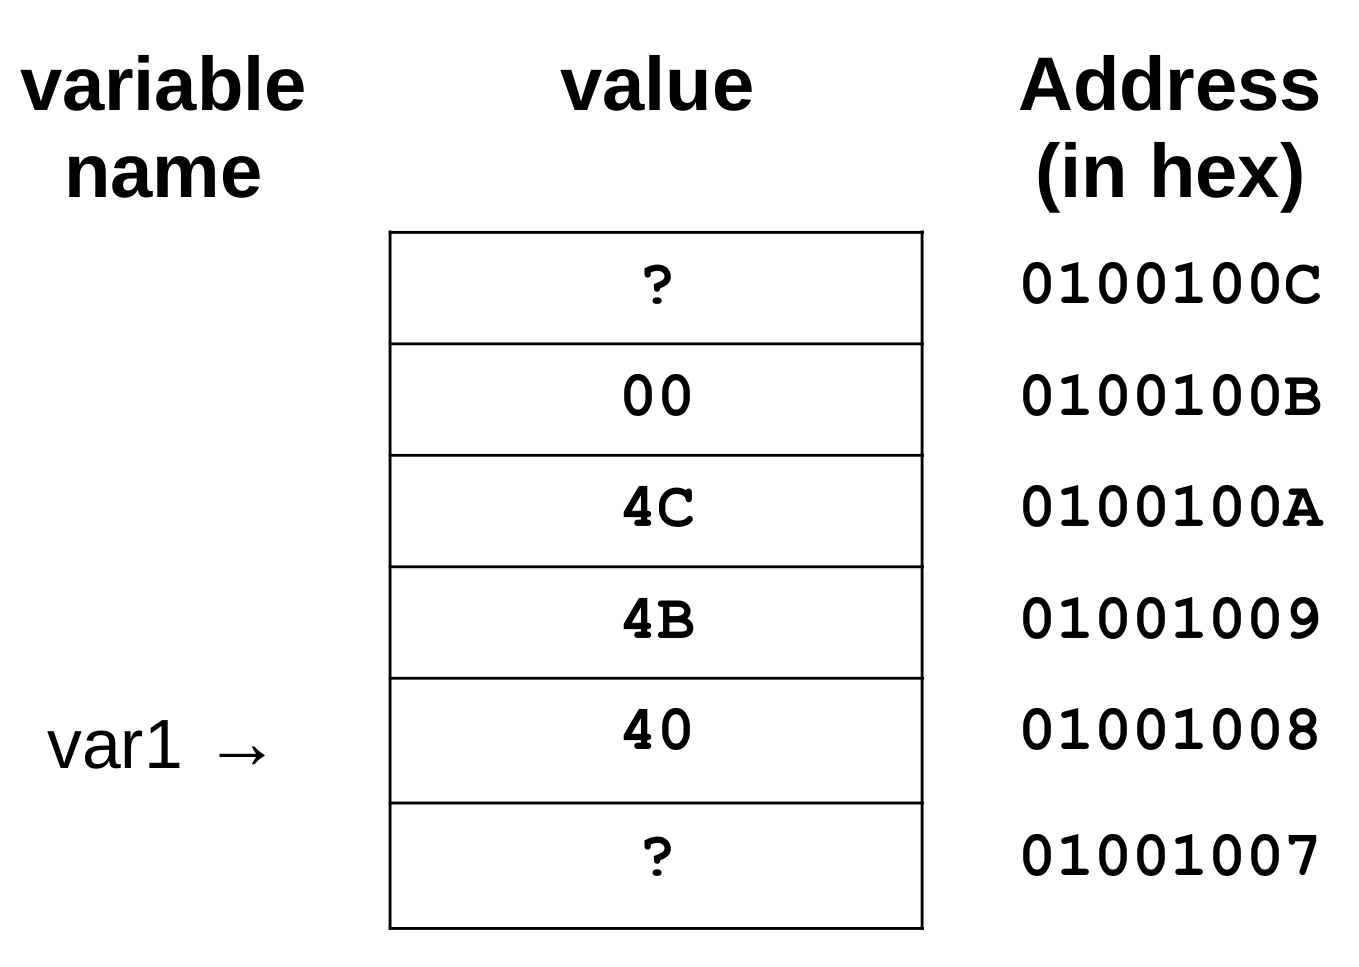
\includegraphics[width=0.8\linewidth]{imagens/littleendien}
	\end{center}
	\caption{Layout de dados Little-Endien}
	\label{fig:littleendien}
\end{figure}

Com base na arquitetura \textit{little-endian}, o \textbf{LSB} é armazenado no endereço de memória mais baixo e o \textbf{MSB} é armazenado no local de memória mais alto.

\section{Layout de memória}
O layout geral da memória para um programa é mostrado na Figura \ref{fig:memlayout}.
\begin{figure}[ht]
	\begin{center}
		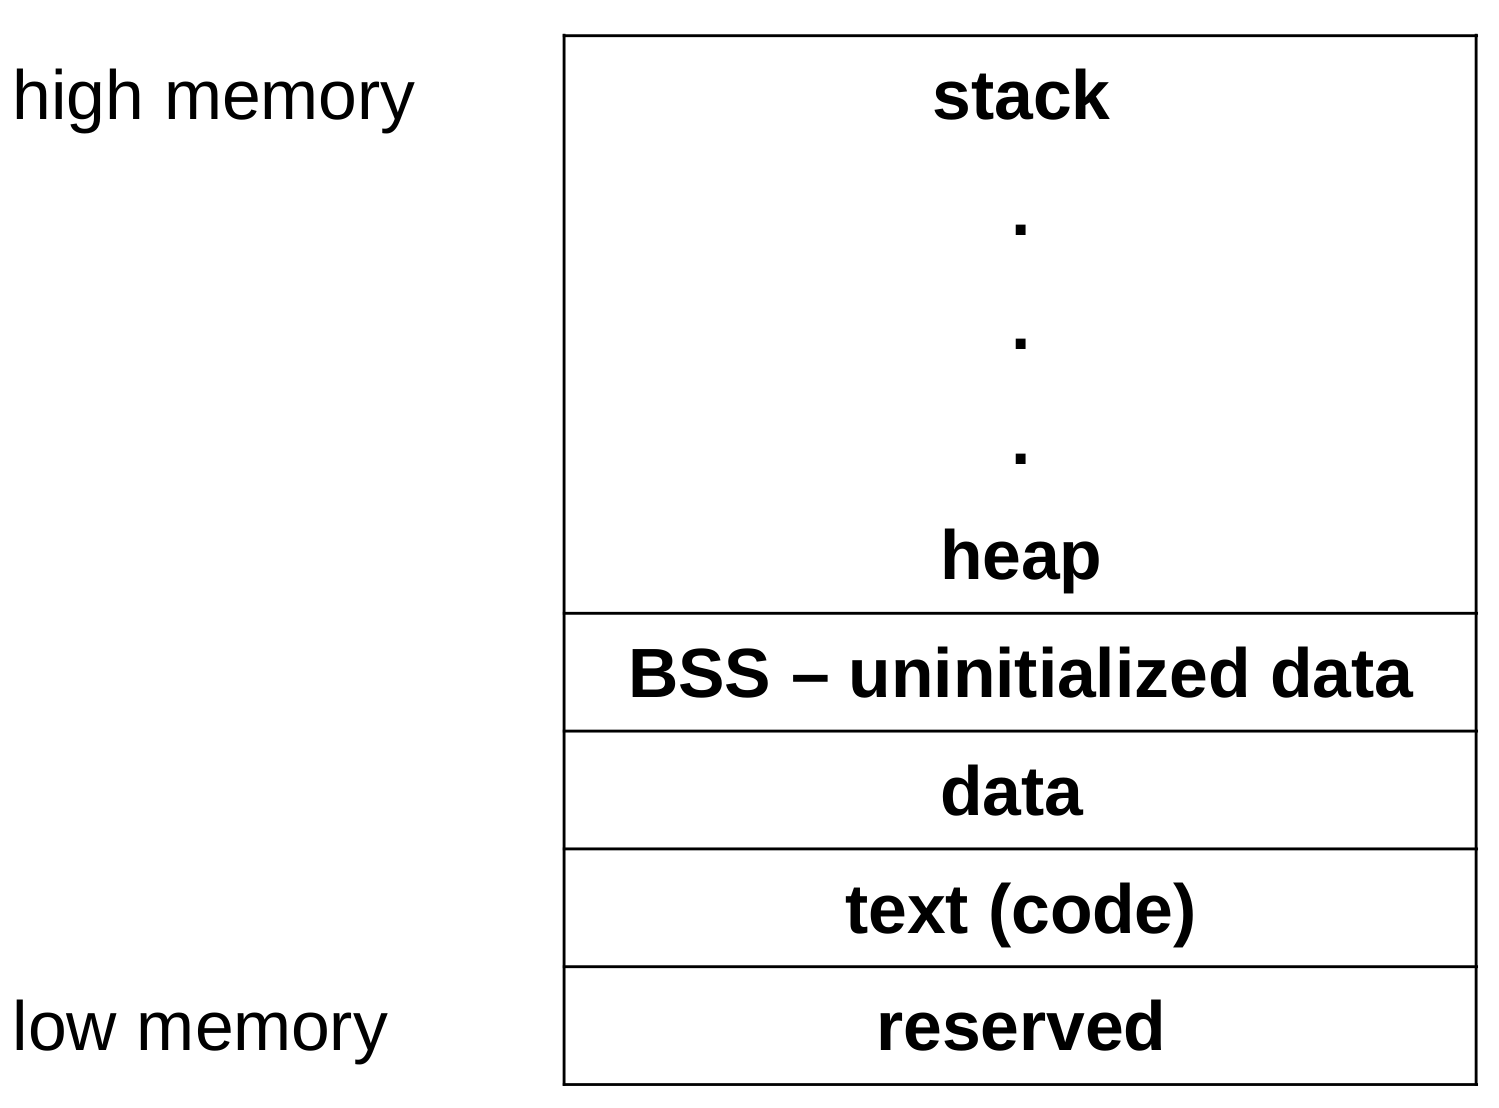
\includegraphics[width=0.8\linewidth]{imagens/memlayout}
	\end{center}
	\caption{Layout geral de memória}
	\label{fig:memlayout}
\end{figure}

A seção reservada não está disponível para programas do usuário. A seção de texto (ou código) é onde a linguagem de máquina\footnote{Para obter mais informações, consulte: https://pt.wikipedia.org/wiki/Código\_de\_máquina} (ou seja, os \textbf{1s} e \textbf{0s} que representam o código) é armazenada. A seção de dados é onde os dados inicializados são armazenados. Isso inclui variáveis declaradas que receberam um valor inicial no momento da montagem. A seção de dados não inicializada, normalmente chamada de seção BSS, é onde as variáveis declaradas que não receberam um valor inicial são armazenadas. Se acessado antes de ser definido, o valor não será significativo. O \textit{heap} é onde os dados alocados dinamicamente serão armazenados (se solicitados). A pilha (stack) começa com muita memória e cresce para baixo.

As seções posteriores fornecerão detalhes adicionais para as seções de texto e dados.


\section{Hierarquia de Memória}
A fim de compreender completamente os vários níveis de memória diferentes e uso associado, é útil revisar a hierarquia de memória\footnote{Para obter mais informações, consulte: \href{https://pt.wikipedia.org/wiki/Hierarquia\_de\_mem\%C3\%B3ria}{Hierarquia de Memória, na Wikipedia}}. Em termos gerais, a memória mais rápida é mais cara e os blocos de memória mais lentos são menos caros. Os registros da CPU são pequenos, rápidos e caros. Os dispositivos de armazenamento secundários, como unidades de disco e unidades de estado sólido (Solid State Devices, SSDs), são maiores, mais lentos e mais baratos. O objetivo geral é equilibrar desempenho e custo.

Uma visão geral da hierarquia da memória é dada na Figura \ref{fig:hierarquia}:
\begin{figure}[ht]
	\begin{center}
		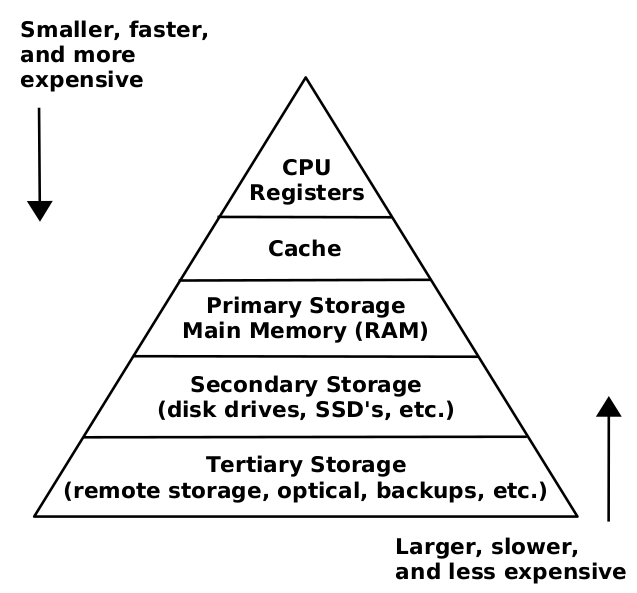
\includegraphics[width=0.8\linewidth]{imagens/hierarquia}
	\end{center}
	\caption{Hierarquia de memória}
	\label{fig:hierarquia}
\end{figure}

Onde o topo do triângulo representa a memória mais rápida, menor e mais cara. À medida que descemos os níveis, a memória se torna mais lenta, maior e menos cara. O objetivo é usar um equilíbrio eficaz entre a memória pequena, rápida e cara e a memória grande, mais lenta e barata.

Algumas características típicas de desempenho e tamanho são as dadas na Tabela \ref{tab:desempenho}:
\begin{table}[h]
	\centering
	\begin{tabular}{|l|l|l|}
		\hline
		\rowcolor[HTML]{C0C0C0} 
		\textbf{Unidade} & \textbf{Exemplo} & \textbf{Velocidade} \\ 
		\rowcolor[HTML]{C0C0C0} 
		\textbf{de Memória} & \textbf{de tamanho} & \textbf{Típica} \\ 
		Registradores & Registradores de  & $  \sim1 $ ns\\ 
		& 16, 64 bits &\\ \hline
		Memória cache & 4 - 8+ Megabytes  & $  \sim5-60 $ ns\\ 
		& (L1 e L2)& \\ \hline
		Armazenamento primário & 2 – 32+ Gigabytes & $  \sim100-150 $ ns\\ 
		 (i.e, memória principal) & &\\ \hline
		Armazenamento secundário  & 500 Gigabytes --  & $  \sim3-15 $ ms\\ 
		(i.e, disco, SSDs, etc.) & 4+ Terabytes& \\\hline
	\end{tabular}
	
	\caption{Desempenho e tamanho de memórias.}
	\label{tab:desempenho}
\end{table}

Com base nesta tabela, um acesso ao armazenamento primário em 100 nanossegundos ($ 100 \times 10^{-9} $) é 30.000 vezes mais rápido do que um acesso ao armazenamento secundário, em 3 milissegundos ($ 3 \times ́10^{-3} $).

As velocidades típicas melhoram com o tempo (e já estão desatualizadas). O ponto chave é que a diferença relativa entre cada unidade de memória é significativa. Essa diferença entre as unidades de memória se aplica mesmo quando \textbf{SSDs} mais novos e mais rápidos estão sendo utilizados.

\section{Exercícios}
Abaixo estão algumas perguntas baseadas neste capítulo.

\subsection{Questionário}
\begin{enumerate}
	\item Faça um desenho da Arquitetura de Von Neumann.
	\item  Qual componente de arquitetura conecta a memória à CPU?
	\item  Onde os programas são armazenados quando o computador é desligado?
	\item  Onde os programas devem ser localizados durante a execução?
	\item  Como a memória cache ajuda no desempenho geral?
	\item  Quantos bytes um inteiro C ++ declarado com a declaração \textbf{int} usa?
	\item  Na arquitetura \textit{Intel X86-64}, quantos \textbf{bytes} podem ser armazenados em cada endereço?
	\item Dado o hexadecimal de 32 bits $ 004C4B40_{16} $, qual é:
	\begin{enumerate}
		\item Byte menos significativo (LSB)
		\item Byte mais significativo (MSB)
	\end{enumerate}
    \item Dado o hexadecimal de 32 bits $ 004C4B40_{16} $, mostre o layout de memória \textit{little-endian} mostrando cada byte na memória.
	\item  Faça um desenho do layout do registrador \textbf{rax}.
	\item  Quantos bits cada um dos seguintes representa:
	\begin{enumerate}
		\item al
		\item rcx
		\item bx
		\item edx
		\item r11
		\item r8b
		\item sil
		\item r14w
	\end{enumerate}
    \item Qual registrador aponta para a próxima instrução a ser executada?
    \item Qual registrador aponta para o topo da pilha atual?
    \item Se \textbf{al} é definido como $ 05_{16} $ e \textbf{ax} é definido como $ 0007_{16} $, \textbf{eax} é definido como $ 00000020_{16} $, e \textbf{rax} é definido
    a $ 0000000000000000_{16} $, mostrar o conteúdo final completo do registro rax inteiro.
    \item Se o registro \textbf{rax} for definido como $ 81.985.529.216.486.895_{10} $ ($ 123456789ABCDEF_{16} $), qual é o conteúdo dos seguintes registros em hexadecimal?
    \begin{enumerate}
    	\item al
    	\item ax
    	\item eax
    	\item rax
    \end{enumerate}
\end{enumerate}